\documentclass[tikz, border=15pt]{standalone}
\usetikzlibrary{positioning, arrows.meta, shapes.geometric}

\usepackage[T1]{fontenc}
\usepackage[utf8]{inputenc}

\begin{document}
	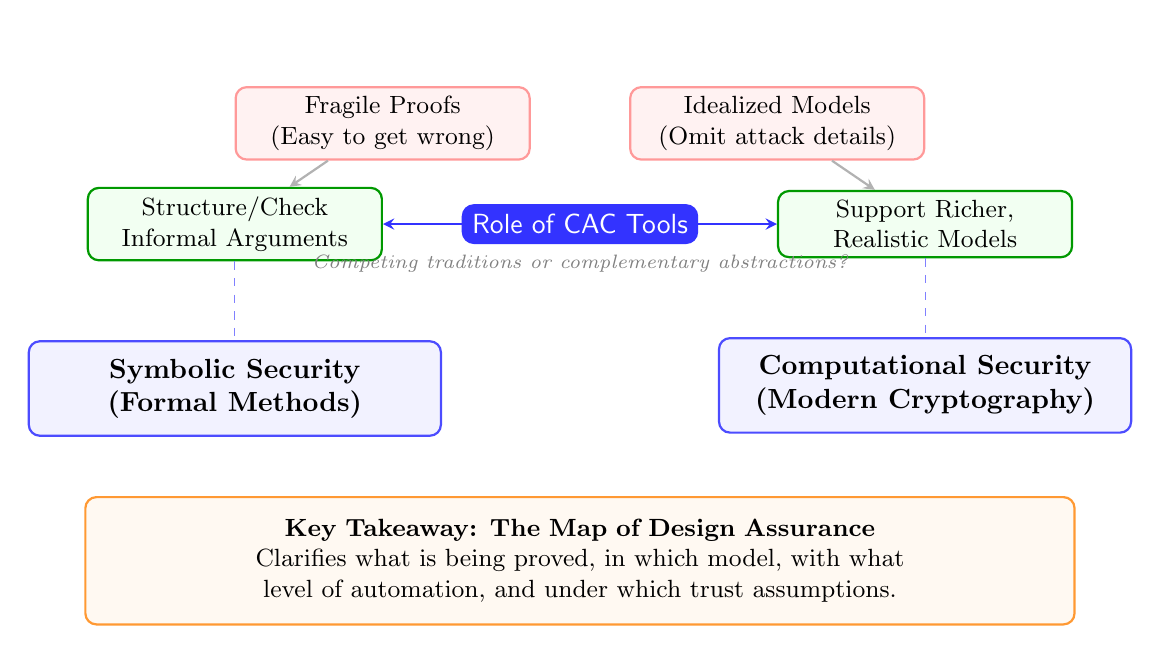
\begin{tikzpicture}[
		>=stealth, font=\sffamily,
		% Define styles
		base/.style={rectangle, rounded corners, thick, align=center},
		header/.style={base, draw=gray!80, fill=gray!10, minimum width=12cm, font=\large\bfseries},
		problem/.style={base, draw=red!40, fill=red!5, text width=3.5cm, font=\small},
		solution/.style={base, draw=green!60!black, fill=green!5, text width=3.5cm, font=\small},
		tradition/.style={base, draw=blue!70, fill=blue!5, text width=5cm, minimum height=1.2cm, font=\bfseries},
		takeaway/.style={base, draw=orange!80, fill=orange!5, text width=12cm, inner sep=8pt, font=\small},
		divider/.style={draw=gray!30, dashed, thick}
		]
		
		% 1. Header
		\node[] (title) {};
		
		% 2. The Problems (Top Row)
		\node[problem, below left=0.5cm and 0.5cm of title] (fragile) {Fragile Proofs\\(Easy to get wrong)};
		\node[problem, below right=0.5cm and 0.5cm of title] (idealized) {Idealized Models\\(Omit attack details)};
		
		% 3. The CAC Pivot
		\node[base, draw=blue!80, fill=blue!80, text=white, below=2cm of title] (cac) {Role of CAC Tools};
		
		% 4. The Solutions (Middle Row)
		\node[solution, left=1cm of cac] (structure) {Structure/Check\\Informal Arguments};
		\node[solution, right=1cm of cac] (richer) {Support Richer,\\Realistic Models};
		
		% Arrows from Problems to Solutions via CAC
		\draw[->, thick, gray!60] (fragile) -- (structure);
		\draw[->, thick, gray!60] (idealized) -- (richer);
		\draw[->, thick, blue!80] (cac) -- (structure);
		\draw[->, thick, blue!80] (cac) -- (richer);
		
		% 5. The Two Traditions (Bottom Row)
		\node[tradition, below=1cm of structure] (symbolic) {Symbolic Security\\(Formal Methods)};
		\node[tradition, below=1cm of richer] (computational) {Computational Security\\(Modern Cryptography)};
		
		% Central label for traditions
		\node[font=\scriptsize\itshape, gray] at ([yshift=-0.5cm]cac) {Competing traditions or complementary abstractions?};
		
		% 6. Key Takeaway Footer
		\node[takeaway, below=1cm of cac, yshift=-2.2cm] (footer) {
			\textbf{Key Takeaway: The Map of Design Assurance}\\
			Clarifies what is being proved, in which model, with what level of automation, 
			and under which trust assumptions.
		};
		
		% Final Connections
		\draw[dashed, blue!50] (structure) -- (symbolic);
		\draw[dashed, blue!50] (richer) -- (computational);
		
	\end{tikzpicture}
\end{document}